\section{Ambiente informatico}
Negli ultimi anni c'è stata una grande evoluzione nell'ambiente informatico e i diversi ambienti (la casa, l'ufficio) sono ora una complessa rete di computer.

I dispositivi mobile si sono arricchiti nelle funzionalità fino al punto da essere indistinguibili dai computer.

\spacer
Questi dispositivi, ogniuno con il suo processore e memoria locali, è connesso da una rete di comunicazione:
\begin{sitemize}
    \item Wide Area Network (WAN)
    \item Metropolitan Area Network (MAN)
    \item Local Area Network (LAN)
    \item Personal Area Network (PAN)
\end{sitemize}

\spacer
Un sistema distribuito ha parecchi vantaggi, infatti può fornire agli utenti un'elaborazione più rapida e può fornire una maggior quantità di dati.

\begin{figure}[H]
    \begin{minipage}{0.55\textwidth}
        \subsubsection*{Modello Client-Server}
        I dispositivi sono i client e richiedono servizi a server. I server permettono l'accesso a servizi e risorse.
    \end{minipage}
    \hfill
    \begin{minipage}{0.35\textwidth}
        \begin{figure}[H]
            \centering
            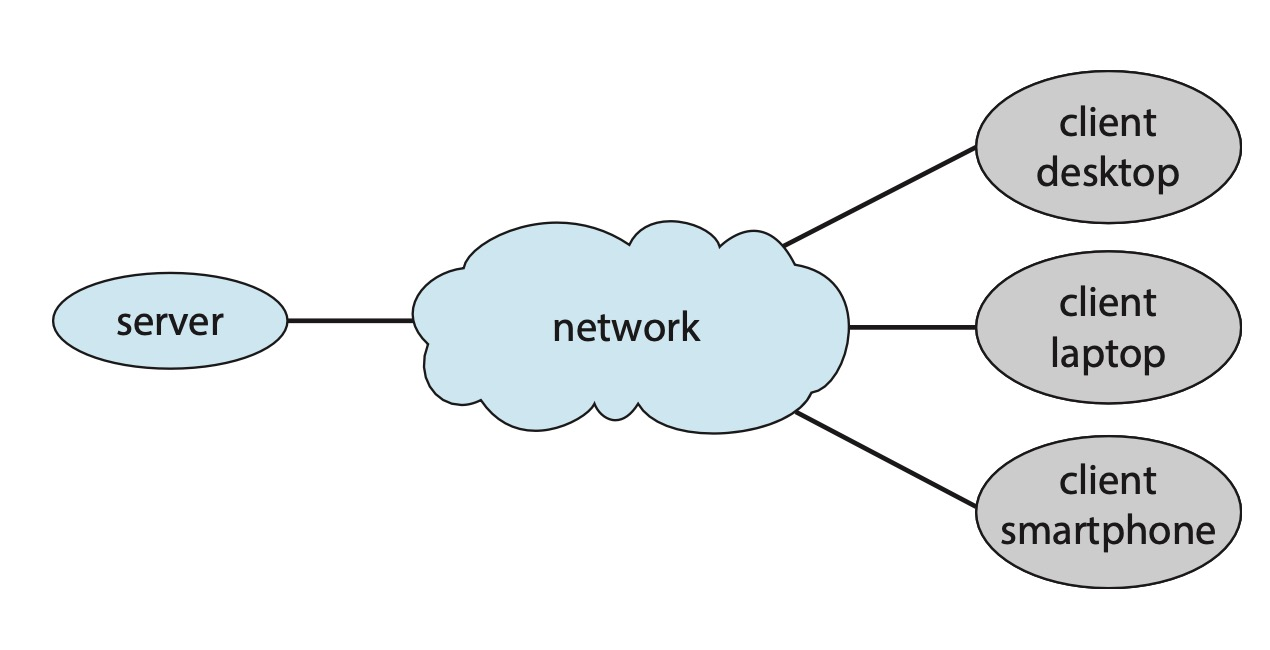
\includegraphics[width=1\linewidth]{assets/client-server.jpg}
        \end{figure}
    \end{minipage}
\end{figure}

\begin{figure}[H]
    \begin{minipage}{0.55\textwidth}
        \subsubsection*{Modello Peer to peer}
        Un modello distribuito peer to peer non fa distinzioni tra client e server, è invece costituita da nodi equivalenti che fungono sia da client che da server rispetto agli altri elementi della rete.

        \spacer

        Quando un nuovo dispositivo vuole entrare in un network peer to peer deve registrare il suo servizio in un registro centralizzato di consultazione della rete. Quando un nodo vuole connettersi con un'altro della rete deve prima contattare il registro centralizzato.
    \end{minipage}
    \hfill
    \begin{minipage}{0.35\textwidth}
        \begin{figure}[H]
            \centering
            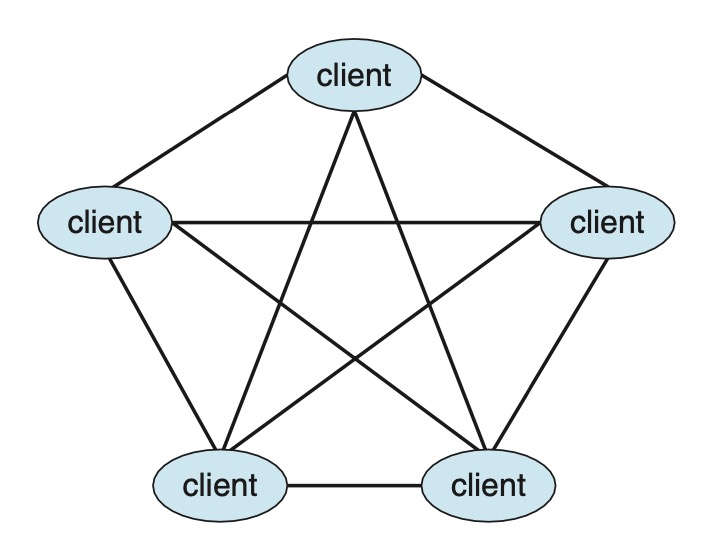
\includegraphics[width=0.9\linewidth]{assets/peer-to-peer.jpg}
        \end{figure}
    \end{minipage}
\end{figure}

\subsubsection*{Cloud Computing}
Il cloud computing è una teconologia che permette di accedere a risorse computazionali, di storage e di applicazione attraverso i servizi di rete.
Risulta particolarmente utile e comodo su dispositivi mobili, le cui risorse sono fortemente limitate.

\spacer
\begin{sitemize}
    \item \textbf{Cloud Pubblico:} liberamente disponibile tramite internet a chi si abbona al servizio
    \item \textbf{Cloud Privato:} gestito da un'azienda per utilizzo interno.
    \item \textbf{Cloud Ibrido:} contiene componenti pubbliche e private.
    \item \textbf{Infrastructure as a service (IaaS):} server o memoria disponibili attraverso l'internet.
    \item \textbf{Platform as a service (PaaS):} un ambiente software il cui hardware viene gestito e che permette di costruire applicativi facilmente.
    \item \textbf{Software as a Service (SaaS):} un'applicazione fruibile tramite internet (es. google docs).
\end{sitemize}

\begin{figure}[H]
    \centering
    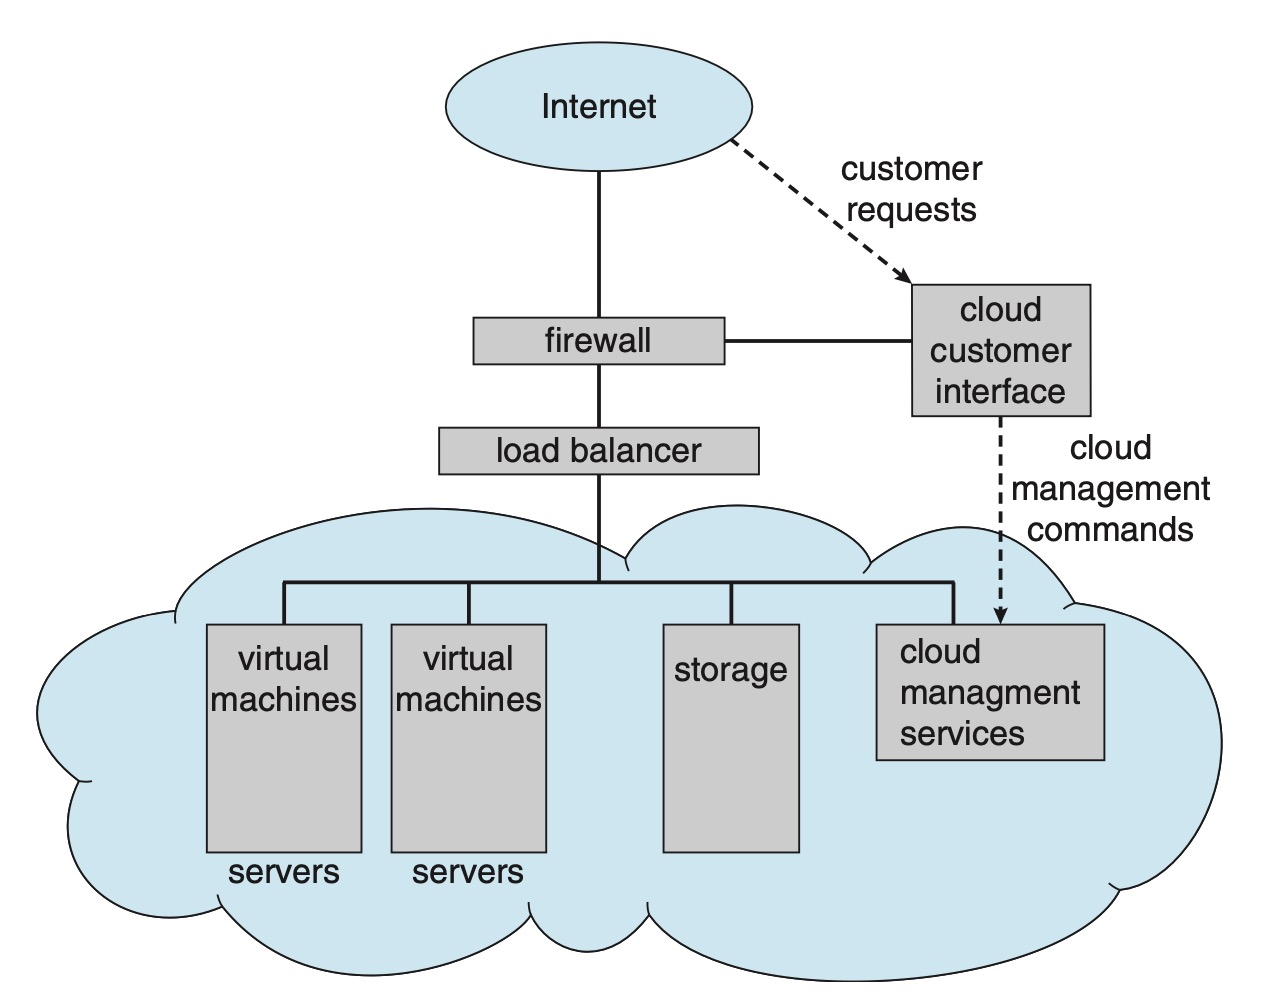
\includegraphics[width=0.35\linewidth]{assets/cloud-computing.jpg}
\end{figure}

\subsubsection*{Sistemi embedded}
Sono gli elaboratori largamente più diffusi, si possono trovare ovunque nelle nostre case.

Sono sistemi rudimentali, hanno compiti precisi, funzionalità limitate e un'interfaccia utente minimale, se presente.

\spacer
Possiamo trovare una grande variabilità tra i sistemi embedded:
\begin{sitemize}
    \item Alcuni sono \textbf{general-purpose} con un sistema operativo standard e delle applicazioni create appositamente per implementare una funzionalità.
    \item Microprocessori con un sistema operativo \textbf{special-purpose} che implementa solamente la funzionalità.
    \item Altri ancora hanno solamente dei \textbf{circuiti} costruiti appositamente per la funzionalità e sono privi di sistema operativo.
    \item \textbf{Sistemi Operativi Real-time}
\end{sitemize}

\spacer
Questi ultimi sono la tipologia più diffusa di sistemi embedded, si utilizza quando il tempo a disposizione per la lettura, l'elaborazione dei dati e l'esecuzione è fissato.

Nel caso in cui il sistema non riesca a produrre una risposta nel tempo prefissato essa verrà considerata errata.
